\section{Multi-class Recognition Policy} \label{sec:tech}
\begin{figure}[h!]
\center{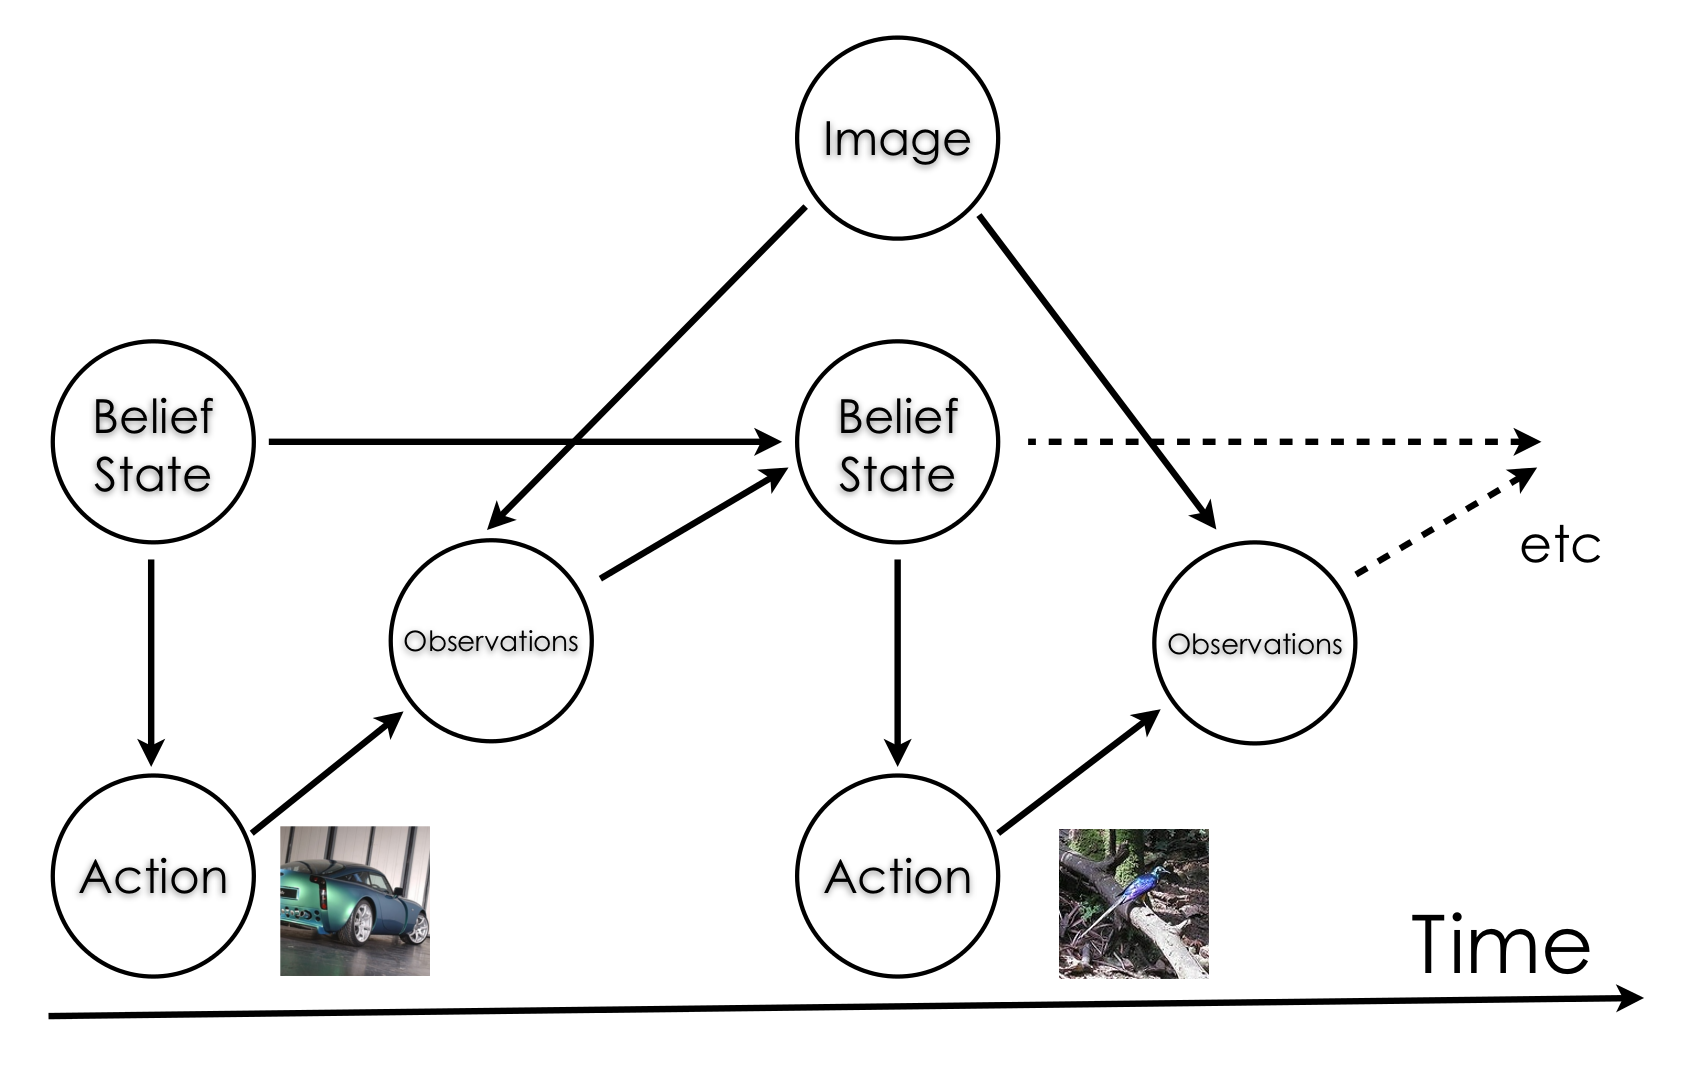
\includegraphics[width=0.66\linewidth]
    {../figures/pomdp.png}}
  \caption{Summary of our approach to the problem. Our system has two major parts: (1) selecting an action by predicting its value; (2) updating the belief state with observations resulting from the action.}
  \label{fig:pomdp}
\end{figure}

Our goal is a multi-class recognition policy $\pi$ that takes an image $\mathcal{I}$ and outputs a list of multi-class detection results by running detector and other \emph{actions} sequentially.

The policy repeatedly selects an action $a_i \in \mathcal{A}$, executes it, receiving observations $o_i$, and then selects the next action.
The set of actions $\mathcal{A}$ can include both classifiers and detectors: anything that would be useful for inferring the contents of the image.

Each action $a_i$ has an expected cost $c(a_i)$ of execution.
Depending on the setting, the cost can be defined in terms of algorithmic runtime analysis, an idealized property such as number of \emph{flops}, or simply the empirical runtime on specific hardware.
We take the empirical approach: every executed action advances $t$, the \emph{time into episode}, by its empirical runtime.

As shown in Figure~\ref{fig:evaluation}, the system is given two times: the setup time $T_s$ and deadline $T_d$.
From the setup time to the deadline, we want to obtain the best possible answer if stopped at any given time.
This corresponds to the general notion of \emph{Anytime} algorithms, and is motivated by desired flexibility in the system.

A single-number metric that corresponds to this objective is simply the ratio of the area captured under the curve to the total area between the start and deadline bounds.
We evaluate policies by this more robust metric and not simply by the final performance at deadline time for the same reason that Average Precision is used instead of a fixed Precision vs. Recall point.

\subsection{Sequential Execution}
An ``open-loop'' policy takes actions in a sequence that does not depend on observations received from previous actions.
The common classifier cascade \cite{Viola2001} is an example.
In contrast, our goal is to learn a dynamic, or ``closed-loop,'' policy, which would exploit the signal in inter-object and scene context for a maximally efficient path through the actions.

The basis for the decisions made by the decision process is called the \emph{state}.
The state, $b$, includes the currently believed distribution over class presence variables $P(\mathbf{C}) = P(C_1, \dots, C_K)$, where we write $P(C_k)$ to mean $P(C_k=1)$

Additionally, the state records the fact that an action $a_i$ has been taken by adding it to the initially empty set $\mathcal{O}$ and recording the resulting observations $o_i$.
We refer to the current set of observations as $\mathbf{o} = \{o_i | a_i \in \mathcal{O}\}$.
The state also includes the time into episode $t$, and the setup and deadline times $T_s,T_d$.

A recognition \emph{episode} takes an image $\mathcal{I}$ and proceeds from the initial state $b^0$ and action $a^0$ to the next pair $(b^1,a^1)$, and so on until $t$ exceeds $T_d$.
At that point, the policy is terminated and a new episode begins on a new image.

The policy's performance at time $t$ is determined by the detections that are part of the set of observations $\mathbf{o}$ at the last state $b^j$ before $t$.
Detection results of unobserved classes are an empty set.

\begin{table}[h!]
\centering
\caption{Summary of the notation.}
\label{tab:notation}
\begin{tabular}{|l|l|}
  \hline
  $\mathcal{I}$ & image \\
  $C_k$         & presence of class $k \in \{1,\dots,K\}$ \\ 
  $t$           & time into episode \\ 
  $T_s$, $T_d$  & start and deadline times \\ 
  $b^j$         & belief state at step $j$ \\ 
  $\pi$         & policy function, $b \mapsto a \in \mathcal{A}$ \\
  $\mathcal{A}$ & set of actions $a$\\ 
  \comment{$\mathcal{F}$ & set of featurization actions \\}
  \comment{$\mathcal{L}$ & set of classification actions\\}
  $o_i$         & a real-valued observation upon executing $a_i \in \mathcal{A}$\\
  $\mathcal{O}$ & set of executed actions\\
  $\mathbf{o}$  & set of observations $\{o_i | a_i \in \mathcal{O}\}$\\
  $c(a_i)$        & cost of executing $a_i$, in units of $t$\\
  \hline
\end{tabular}\end{table}

\subsection{Selecting actions based on expected reward} \label{sec:value}
As our goal is to pick actions dynamically, we want a function $V(b,a): B \times \mathcal{A} \mapsto \mathbb{R}$, where $B$ is the space of all possible states, to assign a value to a potential action, given the current state of the decision process.
We can then define the desired policy $\pi$ as simply taking the (untaken) action with the maximum value:
\begin{align}
\pi(b) = \argmax_{a_i \in \mathcal{A} \setminus \mathcal{O}} V(b,a_i)
\end{align}

This formulation can represent a closed-loop policy if the observations $\mathbf{o}$ (part of the state $b$) play a role in determining the value of a potential action.

Before proceeding, we note that that although the action space $\mathcal{A}$ is quite manageable, consisting of the detectors and classifier we would like to run on the image, the space of possible states $B$ is infinite.
Therefore we cannot learn a tabular representation of $V(b,a)$, and so use function approximation to represent it \cite{Sutton1998}.
We featurize the state-action pair and assume linear structure: $V^\pi(b,a) = \theta_\pi^\top  \phi(b,a_i)$.

Rembmer that at each time step, our system is evaluated by properties of the state $b$ (the list of detections and the classification outputs).
The final evaluation metric is a function of the history of execution $h^0=b^0,b^1,\dots,b^J$, with $J$ being the last step of the process with $t \le T_d$.

\todo{rework the below from the persepctive of individual action rewards, not reward of whole history}
Ideally, the value function for a point in the decision process $b^j$ should give the expected value of the final evaluation metric, over all possible histories starting at point $j$:
\begin{align}
V(b^j,a_i) = \mathbb{E}_{h^j \sim P(h^j|b,a_i)}[R(h^j)]
\end{align}

The reward function $R(h^j)$ assigns a real-valued score to a history.
We have considerable flexibility in defining $R$; it does not necessarily have to be directly tied to the final evaluation.

One feature we want the reward function to have is additivity.
Let's say that given deadline $T_d$ and some image, the policy had time to take $J$ actions.
The total reward of a policy $\pi$ starting at state $b^j$ is then defined as the sum of rewards
\begin{equation}
R(h^j) = \sum_{j'=j}^J R(b_j',a^{j'})
\end{equation}

\subsubsection{Reward: area under the AP vs. Time curve}
\begin{figure}[htb]
  \centering
  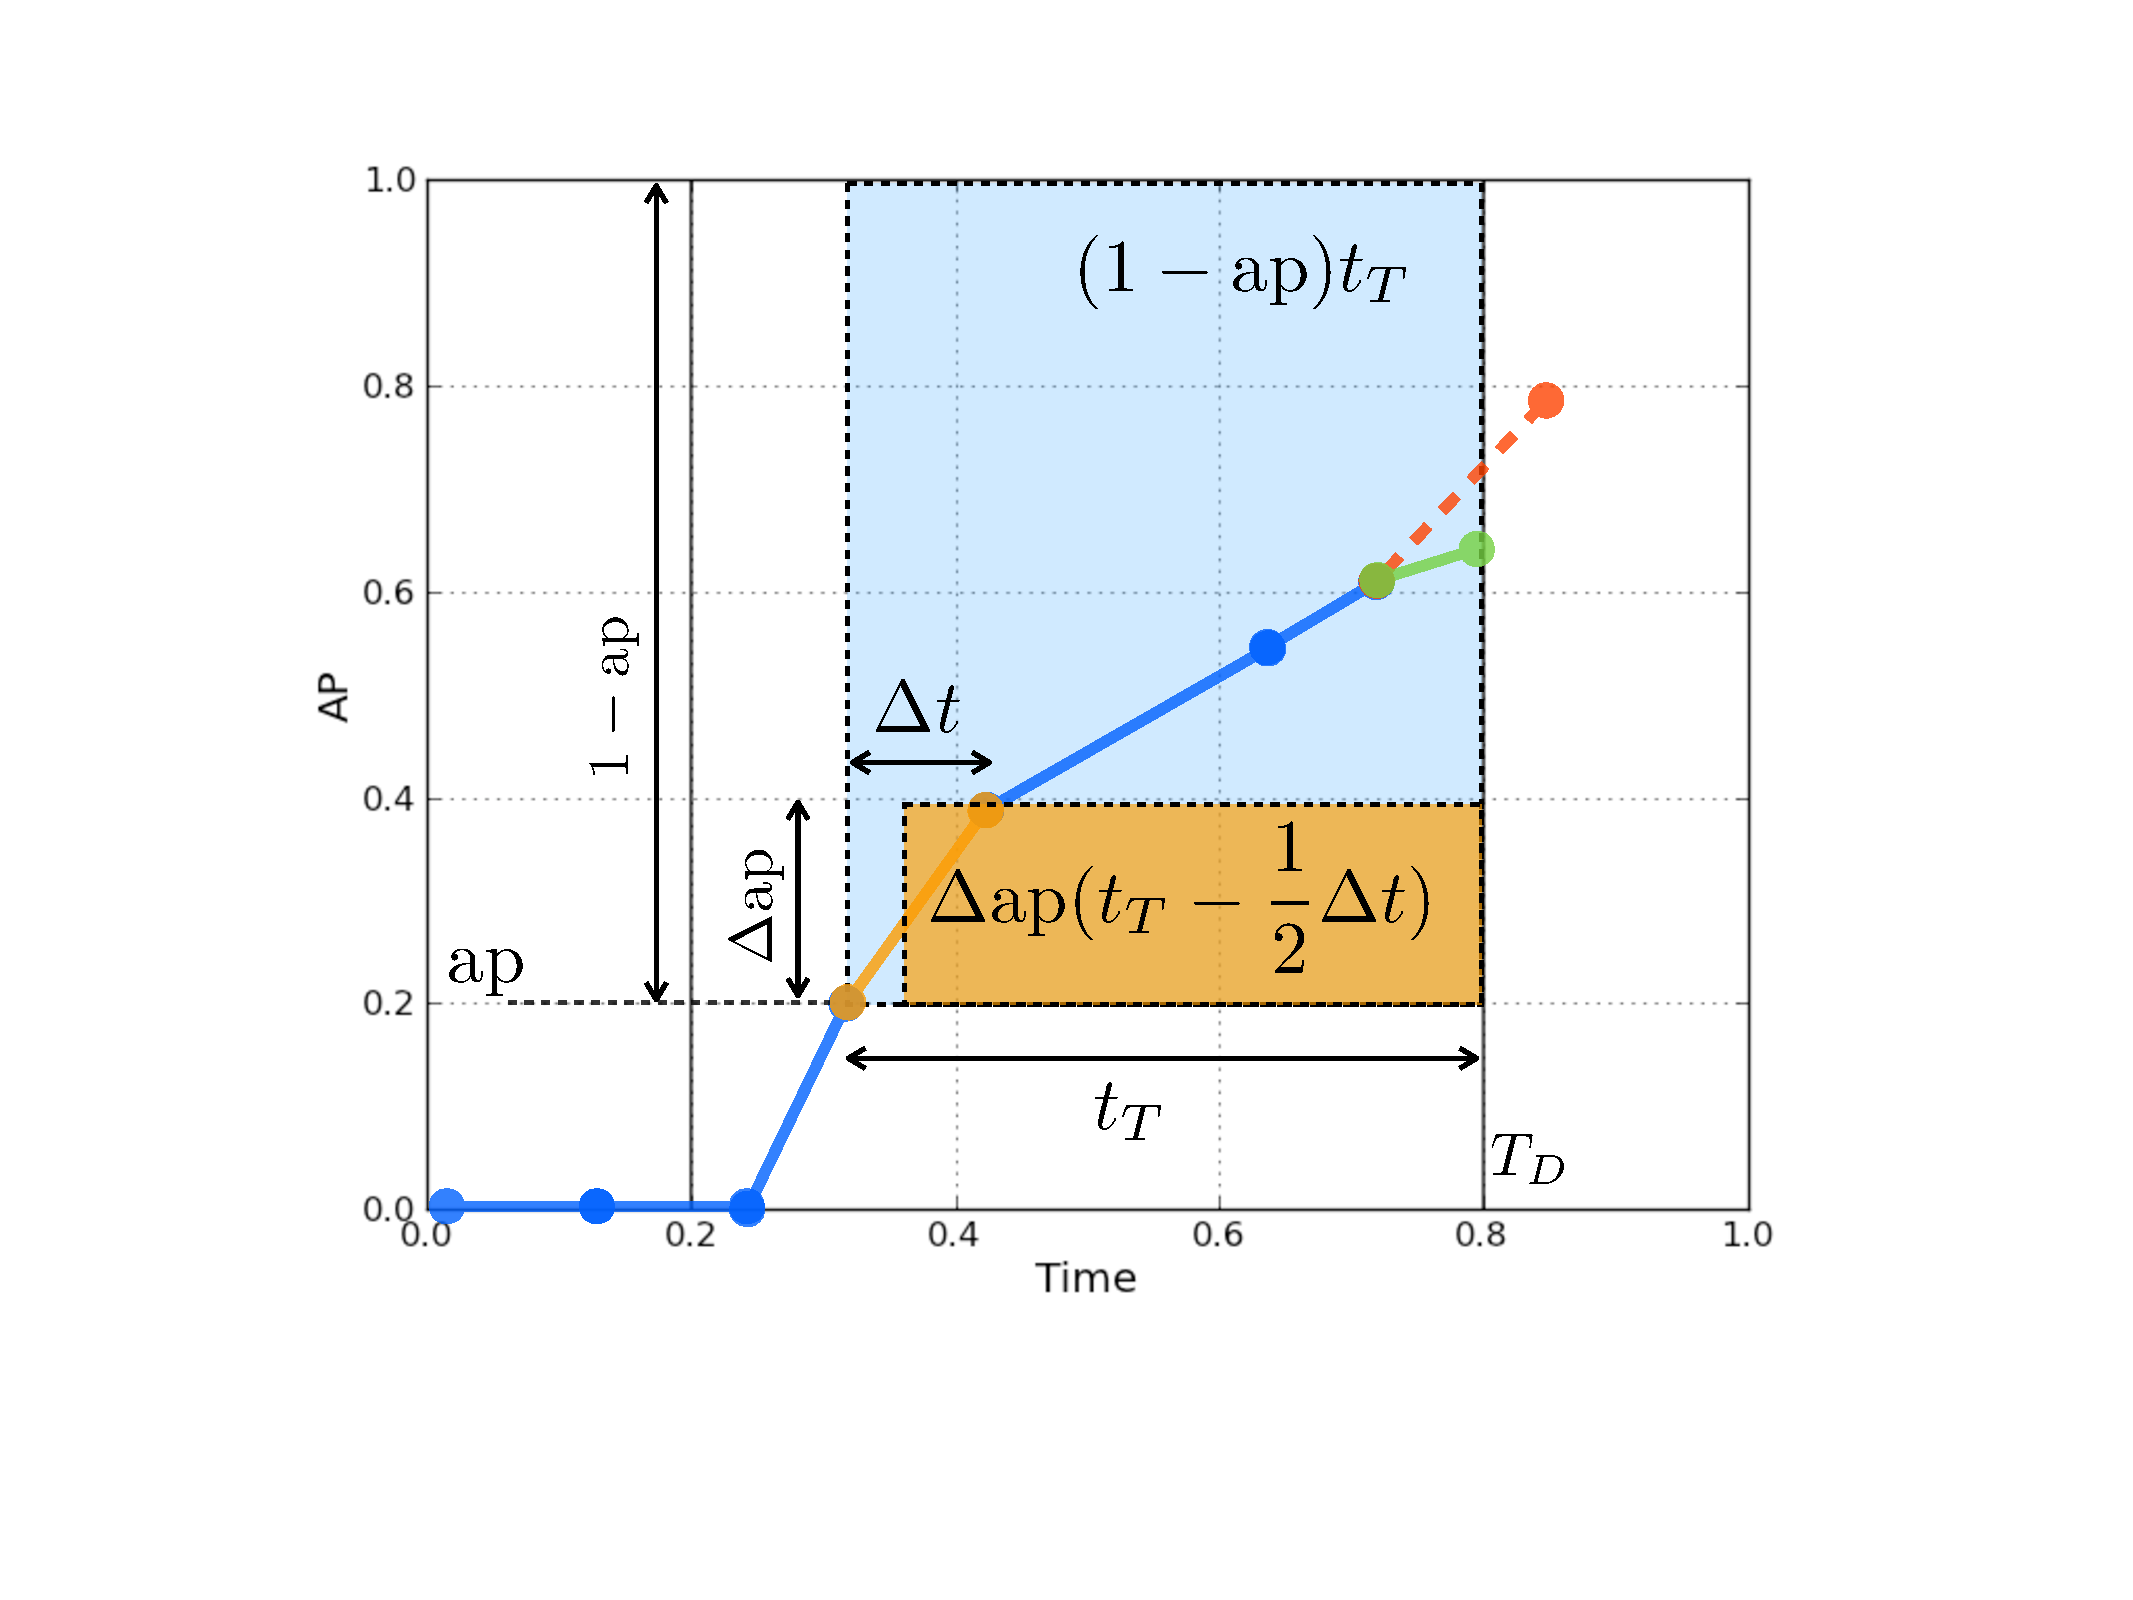
\includegraphics[width=0.56\linewidth]{../figures/apvst_expl.pdf}
  \caption{A per-action greedy value function that corresponds to the maximization of our objective function is the area of the horizontal slice under the curve due to the action. The figure shows this analysis for the action highlighted in orange.}
  \label{fig:rewards}
\end{figure}

The final evaluation of a policy consists of the area under the performance vs. time curve (normalized by the total area).
Accordingly, we formulate per-action rewards such that their addition results in this quantity.

Specifically, as shown in Figure~\ref{fig:rewards}, we define the reward of an action as
\begin{equation}\label{eq:advanced}
R(b^j,a_i) = \frac{\Delta \text{ap}_i (t_T^j-\frac{1}{2}\Delta t_i)}{(1-\text{ap}^j)t_T^j}
\end{equation}
where $t_T^j$ and $\text{ap}^j$ are the time left until deadline and the AP at state $b^j$, and $\Delta t_i$ and $\Delta \text{ap}_i$ are the time taken and AP change produced by the action $a_i$.

The reward is $1$ if the policy takes an action that obtains the maximum possible area under the curve at that point, and $0$ if no area under the curve is captured.

\todo{discuss the raw vs. the normalized area, saying we'll try both}

\subsection{Feature representation and learning the policy}
\todo{write out current approach}

Let us take take the feature representation for an action $a_i$ to be $[P(C_k), \, 1]$, where $C_k$ corresponds to the action.
This corresponds to our heuristic value function, with a bias variable.
The feature representation $\phi(b,a_i)$ then is a vector of size $F|\mathcal{A}|$, with $F=2$ for this feature, where all values are $0$ except those corresponding to $a_i$.

The feature representation of the belief state for a given action $a_i$ that corresponds to class $k$ is defined to be
\begin{align}
\phi_k(b) = [P(C_k), \, H(C_k), \, 1]
\end{align}

Our procedure for learning the weights is standard generalized policy iteration \cite{Sutton1998}.
We first initialize the weights $\theta$ to the heuristic value function of simply picking the maximum $P(C_k)$: $\theta_i = [1, \,0, \,0]$.

With this policy, we run $N$ recognition episodes.
From the state-action samples gathered in running the episodes, we formulate a matrix $\Phi$ from the featurizations $\phi(b^j,a_i)$, and a vector $y$ consisting of the individual rewards $R(b^j,a_i)$.

The rewards are computed as the sum of discounted rewards to the end of the episode:
\begin{align}
R(b^j,a_i) = \sum_{i=0}^{J-j} \lambda^i R(b_{j+i},a^{j+i})
\end{align}
Note that with $\lambda=0$, the reward is determined entirely by the actual action taken; with $\lambda=1$, the reward is the sum of all rewards until the end of the episode.

We then solve the system $\Phi \theta = y$ for $\theta$ with Lasso regression.
With the updated weights $\theta$, we run $N$ more episodes and repeat the procedure until convergence.

The parameters of this training procedure are the $\alpha$ weight on the regularization term in the regression and the $\lambda$ discount weight.
We cross-validate for both values.


\subsection{Updating probabilities}
\begin{figure}[h!]
\centering
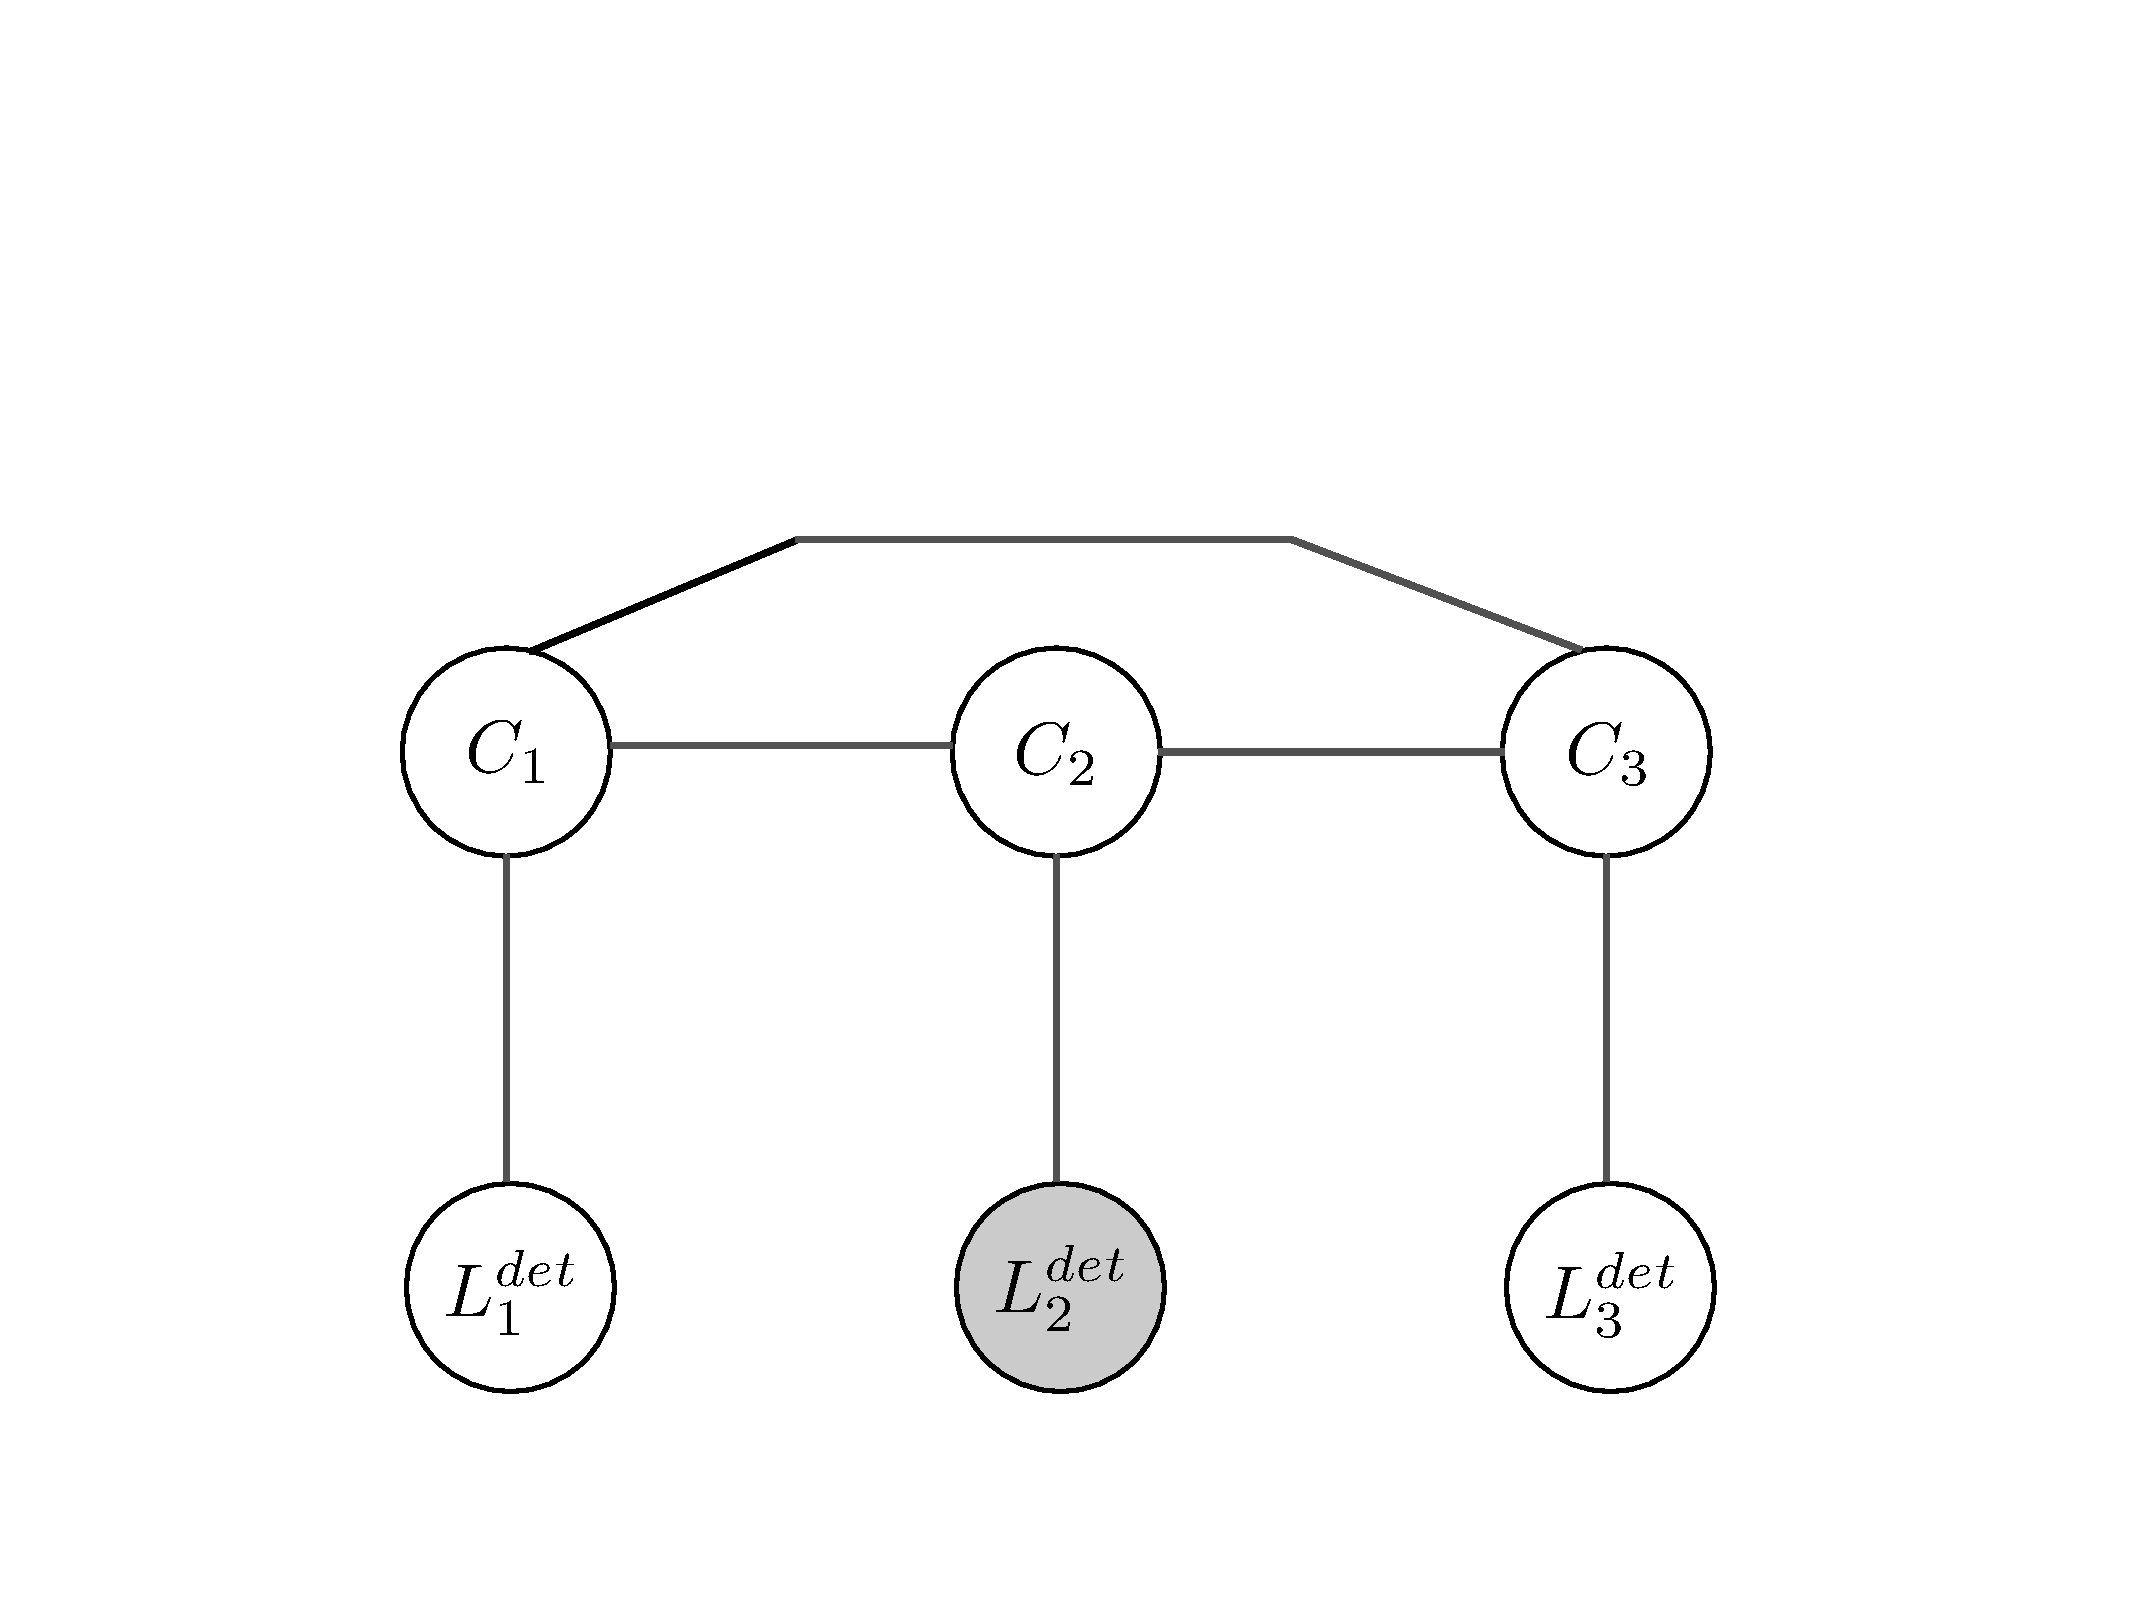
\includegraphics[width=0.56\linewidth]{../figures/inf_model_mrf_1.pdf}
\caption{
The MRF inference model used in our system.
We show a point in the middle of the decision process for 3 classes; one action has already been taken.
\comment{Some classifiers have already been observed.}
}
\label{fig:model}
\end{figure}

\todo{Rework from the persepctive of two potential ways of updating the beliefs with observations: just putting them in directly vs. going through MRF. De-emphasize the need for the model, treat it as an extra oomph.}

The quantities that may be useful to us for selecting which actions to deploy are the probabilities and entropies of the class presence variables $C_k$.
These allow us to look for the most probable classes given the observations.
When the policy starts, the model should present the prior distributions $P(C_k)$; as observations are accrued, the model should present the updated conditionals $P(C_k|\mathbf{o})$.

We employ a pairwise fully-connected Markov Random Field (MRF), as shown in Figure~\ref{fig:model}.
All parameters of the model are trained on fully-observed data.
Exact inference is generally intractable in this model.
Instead, we use Loopy Belief Propagation, which does not provide general convergence guarantees but has been shown to work well empirically on similar tasks \cite{Desai2009}.

The $L_i$ variables are discretized from real-valued responses of a classifier on the detections output by the deformable part-model detector we employ (see Section~\ref{sec:tech}).
The classifier is a linear SVM on the top two max detection scores in the list of detections.
The responses are discretized per variable based on the distribution of the scores on the training dataset.

The graphical model structure is set as fully-connected, but as shown in \autoref{fig:dataset_stats}, some classes are overwhelmingly unlikely to co-occurr.
Accordingly, the graph edge weights are learned with L1 regularization, which obtains the desired sparse structure \cite{Lee2006}.
 is implemented with an open-source graphical model package \cite{Jaimovich2010}.
 